\begin{frame}
    \frametitle{Upper bounds}

    \begin{itemize}
		\item Linear systems over $\mathbb{F}_2$
			\begin{itemize}
				\item hard for resolution and $\DPLL$;
				\item easy for Linear splitting trees.
			\end{itemize}
        \pause
		\item Perfect matching principle for graphs with odd vertices (\textit{almost} nonlinear example)
			\begin{itemize}
				\item hard for resolution and $\DPLL$ [Razborov 2003, ISS 2015];
				\item easy for Linear splitting trees.
			\end{itemize}
        \pause
		\item Pebbling contradictions (nonlinear example):
			\begin{itemize}
				\item for CNF $\phi$ we denote by $\phi^{\oplus}$ a CNF formula obtained from $\phi$ by substituting $x_1 \oplus
					x_2$ for each variable $x$;
				\item{} [Urquhart, 2011] the size of tree-like Resolution of $\phi^{\oplus}$ is at least $2^{d(\phi)}$, where
					$d(\phi)$ is the minimal depth of the resolution proof of $\phi$;
				\item{} [Urquhart, 2011] pebbling contradictions $Peb(G_n)$ such that $d(Peb(G_n)) = \Omega(n / \log(n))$ and
					$Peb(G_n)$ has $O(n)$ tree-like resolution proof;
				\item Tree-like resolution proof of $Peb^\oplus(G_n)$ is at least $2^{n / \log n}$, while $Peb^\oplus(G_n)$ has $O(n)$-size LST. 
			\end{itemize}
	\end{itemize}
\end{frame}




\begin{frame}
    \frametitle{Linear systems}

    \begin{columns}
		\begin{column}{1cm}
			Unsatisfiable system:

			$\left\{ \begin{aligned}
				f_1 = \alpha_1 \\
				f_2 = \alpha_2 \\
				\dots\\
				f_m = \alpha_m
			\end{aligned}\right.$
		\end{column}


		\begin{column}{9cm}
			\tikzstyle{end} = [thin, circle, minimum size = 0.1cm, draw, inner sep = 0.1pt]
\tikzstyle{leaf} = [thin, circle, minimum size = 0.6cm, draw, inner sep = 0.1pt, blue]
            
\tikzstyle{level 1}=[level distance = 1.5cm, sibling distance = 1.5cm]
\tikzstyle{level 2}=[level distance = 1.5cm, sibling distance = 4cm]
\tikzstyle{level 3}=[level distance = 2cm, sibling distance = 1.5cm]
\tikzstyle{level 4}=[level distance = 2cm, sibling distance = 1.3cm]

\tikzstyle{edge from parent} = [thin, draw]

    
\begin{tikzpicture}[label distance = 8mm]
	\node [end] {}
	    child {
        	node {$\vdots$}
           	edge from parent
            node[left] {$f_1 = 1 - \alpha_1$}
        }
        child {
        	node[end] {}
            child {
		        node[end] {}
                child[level distance = 1.cm, sibling distance = 2.5cm] {
        			node[end] {}
                    child[level distance = 1cm] {
                    	node {$\vdots$}
                    	edge from parent[ultra thick]
	        		    node[left] {$x_2 = 0$}
                    }
                    child[level distance = 1cm] {
                    	node {$\vdots$}
                        child[level distance = 1.5cm, sibling distance = 1.8cm] {
                        	node {\alert{no sol.}}
                            edge from parent[ultra thick]
		        		    node[left] {$x_k = 0$}
                        }
                        child[level distance = 1.5cm, sibling distance = 1.8cm] {
                        	node {\alert{$f_2 = \alpha_2$}}
                            edge from parent[ultra thick]
		        		    node[right] {$x_k = 1$}
                        }
                    	edge from parent[ultra thick]
	        		    node[right] {$x_2 = 1$}
                    }
		           	edge from parent[ultra thick]
        		    node[left] {$x_1 = 0$}
		        }
                child[level distance = 1.cm, sibling distance = 2.5cm] {
                  	node {$\vdots$}
                    edge from parent[ultra thick]
                    node[right] {$x_1 = 1$}
                }
	            edge from parent
		        node[left] {$f_2 = 1 - \alpha_2$}
			}
		    child {
		        node[end] {}
                child {
        			node {$\vdots$}
		           	edge from parent
        		    node[left] {}
		        }
                child {
                  	node {$\vdots$}
                    child{
  		                node {$\vdots$}
			           	edge from parent
        			    node[left] {$f_m = 1 - \alpha_m$}
                    }
                    child{
  		                node {\alert{no sol.}}
			           	edge from parent[line width = 2.1pt]
        			    node[right] {$f_m = \alpha_m$}
                    }
                    edge from parent[line width = 2.1pt]
                    node[right] {$f_3 = \alpha_3$}
                }
	            edge from parent[line width = 2.1pt]
		        node[right] {$f_2 = \alpha_2$}
            }
           	edge from parent[line width = 2.1pt]
            node[right] {$f_1 = \alpha$}
        };
\end{tikzpicture}

%%% Local Variables: 
%%% mode: latex
%%% TeX-master: t
%%% End: 

		\end{column}
	\end{columns}

	$f_2 = x_1 + \dots + x_k$
\end{frame}


\begin{frame}
    \frametitle{Lower bound for PHP}

    \begin{itemize}
		\item $PHP^m_n$, $m$ pigeons, $n$ holes;
		\item variables $p_{i, j}$, $i \in [m]$, $j \in [n]$; 
			$p_{i, j}$: $i$-th pigeon is in the $j$-th hole;
		\item clauses:
			\begin{itemize}
				\item \mycolor{blue}{Long} clauses: $p_{i, 1} \lor p_{i, 2} \dots \lor p_{i, n}$ for all $i \in [m]$;
				\item \mycolor{blue}{Short} clauses: $\lnot p_{i, k} \lor \lnot p_{j, k}$ for all $i \neq j \in [m]$ and all $k
					\in [n]$.
			\end{itemize}
		\item $PHP^m_n$ is unsatisfiable iff $m > n$.
	\end{itemize}
    
	\pause

    \begin{theorem}
        The size of any LST of $PHP^m_n$ is at least $2^{\frac{n - 1}{2}}$.
    \end{theorem}

\end{frame}



%\begin{frame}
%    \frametitle{Lower bound for PHP}

%    \begin{theorem}
%        The size of any LST of $PHP^m_n$ is at least $2^{\frac{n - 1}{2}}$.
%    \end{theorem}


%	\mycolor{blue}{Proof.}
%	\begin{columns}
%		\begin{column}{8.5cm}
%			\begin{itemize}
%				\item $\pi$ is \mycolor{blue}{acceptable} if it satisfies all short
%		            clauses.
%               	\pause
%				\item Consider LST $T$ and cut off all vertices without acceptable
%	                solutions. Resulting tree $T'\neq \emptyset$.
%                \pause
%				\item Every leaf in $T'$ refutes some long clause.
%           		\pause
%				\item Consider a path $\ell$ in $T'$ from root to leaf. We claim
%                	that $\ell$ contains at least $\frac{n - 1}{2}$ splitting
%                    points.
%                \pause
%				\item $\Phi_\ell$ is a set of equations followed by splitting points
%	                along $\ell$. $\Phi_\ell$ has no acceptable solutions that sutisfies
%    	            some long clause. 
%			\end{itemize}
%		\end{column}
%		\begin{column}{2cm}
%			\scalebox{0.6}{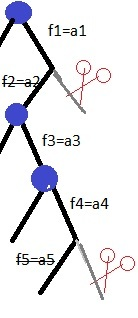
\includegraphics{pics/php.jpg}}
%		\end{column}
%	\end{columns}
    
%	\pause
%    \begin{lemma}
%        Let a linear system $Ap = b$ from variables $p =
%        (p_{i, j})_{i \in [m], j \in [n]}$ have  $k \le \frac{n - 1}{2}$ equations
%        and have an acceptable solution. Then  $\forall i \in [m] \exists \sigma:$
%        $\sigma$ is an acceptable solution and satisfies $p_{i, 1} \lor p_{i, 2} \lor
%        \dots \lor p_{i, n}$.
%    \end{lemma}
%\end{frame}


%%% Local Variables: 
%%% mode: latex
%%% TeX-master: t
%%% End: 
